%%%%%%%%%%%%%%%%%%%%%%%%%%%%%%%%%%%%%%%%%
% Large Colored Title Article
% LaTeX Template
% Version 1.1 (25/11/12)
%
% This template has been downloaded from:
% http://www.LaTeXTemplates.com
%
% Original author:
% Frits Wenneker (http://www.howtotex.com)
%
% License:
% CC BY-NC-SA 3.0 (http://creativecommons.org/licenses/by-nc-sa/3.0/)
%
%%%%%%%%%%%%%%%%%%%%%%%%%%%%%%%%%%%%%%%%%

%----------------------------------------------------------------------------------------
%	PACKAGES AND OTHER DOCUMENT CONFIGURATIONS
%----------------------------------------------------------------------------------------

\documentclass[DIV=calc, paper=a4, fontsize=11pt, twocolumn]{scrartcl}	 % A4 paper and 11pt font size

\usepackage{lipsum} % Used for inserting dummy 'Lorem ipsum' text into the template
\usepackage[english]{babel} % English language/hyphenation
\usepackage[protrusion=true,expansion=true]{microtype} % Better typography
\usepackage{amsmath,amsfonts,amsthm} % Math packages
\usepackage[svgnames]{xcolor} % Enabling colors by their 'svgnames'
\usepackage[hang, small,labelfont=bf,up,textfont=it,up]{caption} % Custom captions under/above floats in tables or figures
\usepackage{booktabs} % Horizontal rules in tables
\usepackage{fix-cm}	 % Custom font sizes - used for the initial
                         % letter in the document
\usepackage{graphicx}
\usepackage{subfig}
\usepackage{cite}

\usepackage{sectsty} % Enables custom section titles
\allsectionsfont{\usefont{OT1}{phv}{b}{n}} % Change the font of all section commands

\usepackage{fancyhdr} % Needed to define custom headers/footers
\pagestyle{fancy} % Enables the custom headers/footers
\usepackage{lastpage} % Used to determine the number of pages in the document (for "Page X of Total")

% Headers - all currently empty
\lhead{}
\chead{}
\rhead{}

% Footers
\lfoot{}
\cfoot{}
\rfoot{\footnotesize Page \thepage\ of \pageref{LastPage}} % "Page 1 of 2"

\renewcommand{\headrulewidth}{0.0pt} % No header rule
\renewcommand{\footrulewidth}{0.4pt} % Thin footer rule

\usepackage{lettrine} % Package to accentuate the first letter of the text
\newcommand{\initial}[1]{ % Defines the command and style for the first letter
\lettrine[lines=3,lhang=0.3,nindent=0em]{
\color{DarkGoldenrod}
{\textsf{#1}}}{}}

%----------------------------------------------------------------------------------------
%	TITLE SECTION
%----------------------------------------------------------------------------------------

\usepackage{titling} % Allows custom title configuration


\newcommand{\HorRule}{\color{DarkGoldenrod} \rule{\linewidth}{1pt}} % Defines the gold horizontal rule around the title

\pretitle{\vspace{-30pt} \begin{flushleft} \HorRule \fontsize{50}{50} \usefont{OT1}{phv}{b}{n} \color{DarkRed} \selectfont} % Horizontal rule before the title

\title{\Huge Text Mining CA Report} % Your article title

\posttitle{\par\end{flushleft}\vskip 0.5em} % Whitespace under the title

\preauthor{\begin{flushleft}\large \lineskip 0.5em \usefont{OT1}{phv}{b}{sl} \color{DarkRed}} % Author font configuration

\author{Li Jingchao(A0134565A), Zhang Fan(a0134457a), Ning
  Chao(A0134563H), Devendra Desale(A0134465E), Pan An(A0134556A) } % Your name

\postauthor{\footnotesize \usefont{OT1}{phv}{m}{sl} \color{Black} % Configuration for the institution name
National University of Technology % Your institution

\par\end{flushleft}\HorRule} % Horizontal rule after the title

\date{} % Add a date here if you would like one to appear underneath the title block

%----------------------------------------------------------------------------------------

\begin{document}

\maketitle % Print the title

\thispagestyle{fancy} % Enabling the custom headers/footers for the first page

%----------------------------------------------------------------------------------------
%	ABSTRACT
%----------------------------------------------------------------------------------------

% The first character should be within \initial{}
\initial{T}\textbf{his report is the project report for Textmining
  Course Accessment.
The given questions described a situation where people are trying to
find a pattern among large amount of cases of accidents in construction
fields.
In this paper we are going to
  explain our proposal and result for  each problem.  }

\tableofcontents % Print the contents section
%----------------------------------------------------------------------------------------
%	ARTICLE CONTENTS
%----------------------------------------------------------------------------------------


\section*{Business Goal}
Despite improvement in recent years, the construction industry remains
the top contributor for workplace fatalities in Singapore. In
construction industry, after a fatal or catastrophic accident happens,
an inspection is conducted in response, generating a report including
a Fatality and Catastrophe Investigation Summary. The summaries
provide a complete description of the incident, generally including
events leading to the incident and causal factors. These summaries can
be analyzed to identify occupations and workplace activities that face
higher safety risks than others. Based on the result of analysis,
construction project managers and safety professionals can then take
appropriate measures to mitigate the identified risks and prevent the
occurrence of similar accidents. All of our tasks are finished with
NLTK~\cite{nltk}.

\section*{Findings}
For each of the data analysis task some new information will be
generated. The following discovery might be interesting:

\begin{itemize}
\item Three of the main reasons that causes fatal injuries to workers
  are:
  \begin{enumerate}
  \item Struck by moving objects
 \item Caught in/between objects
\item Falling from high places
  \end{enumerate}

\item Large amount of fatal accidents involves falling, including
  falling objects and people falling.

\item Almost all the accidents happen to employees and workers.

\end{itemize}

The most common activities were found as working on (something), operating on machines,
installing the equipment.
Current analysis can be extended to performed as per the type of accidents.
Finding the common activities is very complex part, as the activities vary too much and even the
similar activities are written in different ways.
In many cases activity is not mentioned in generic way, this thing causes issue when we want to
drill down to different activities.
\section*{Introduction}
In construction industry, after a fatal or catastrophic accident
happens, an inspection is conducted in response, generating a report
including a Fatality and Catastrophe Investigation Summary. The
summaries provide a complete description of the incident, generally
including events leading to the incident and causal factors. These
summaries can be analyzed to identify occupations and workplace
activities that face higher safety risks than others. Based on the
result of analysis, construction project managers and safety
professionals can then take appropriate measures to mitigate the
identified risks and prevent the occurrence of similar accidents.

This paper proposed methods for text data mining in these tasks. These
methods uses combinations of different methods in natural language
processing:

\begin{enumerate}
\item SVM(for classification)
\item POS Tagging
\item Grammar and Regular Expression
\end{enumerate}

Support vector machine~\cite{svm} is used for basic accident case
classification. Support Vector Machines are very specific class of
algorithms, characterized by usage of kernels, absence of local
minima, sparseness of the solution and capacity control obtained by
acting on the margin, or on number of support vectors, etc.

POS tagging~\cite{pos} is now done in the context of computational linguistics,
using algorithms which associate discrete terms, as well as hidden
parts of speech, in accordance with a set of descriptive tags. In this
paper POS tagging is one of the key component for extracting
information from large amount of messages.




\section{Fatal Accidents}
Practice the concepts and techniques we have learned in Text Mining
elective. Perform text mining on Fatality and Catastrophe
Investigation Summaries. Find out type of accidents (in terms of main
causes) which are more common in fatal or catastrophic accidents. Find
out kinds of objects which cause the accidents. Extract the more risky
occupations in such accidents. Find out the common activities that the
victims were engaged in prior to the accident.

Our method is to use SVM classification method to train and
test a model, then use the model to do classification on type of
accidents (in terms of main causes) on new data. Support Vector
Machine can be applied not only to classification problems but also to
the case of regression. Still it contains all the main features that
characterize maximum margin algorithm: a non-linear function is leaned
by linear learning machine mapping into high dimensional kernel
induced feature space. The capacity of the system is controlled by
parameters that do not depend on the dimensionality of feature space.




\subsection{Data Preprocessing}
%------------------------------------------------
The giving training data quality is not so good. Some of the labels
are not correct. Before doing text mining work, we made some
modifications in the two tables. For this task we mainly used
MsiaAccidentCases.csv. Some of the types are not consistent with the
titles and summary contents. We correct them according to the title
and summary content. Besides there are other and others in the type
list. We change them to other to make it uniform. We corrected almost 24
type of accidents of the records.

\subsection{Classification}
\label{classification}

We use the MsiaAccidentCases.csv data to build the classification
model. There are 3 columns of this data set. During the classification
model building, we use only the cause and summary. Split the
MsiaAccidentCases.csv data into 2 parts, 80\% for training and 20\% for
                                \% testing. Use TF-IDF Vectorizer from
                                \% the data features.
Use SVM algorithm to train the classification model on the 80\% of the MsiaAccidentCases.csv data. Then use the rest 20\% of the data to do testing.


For SVM configuration we set $C = 5000$, $gamma = 0.0$, $kernel =
'rbf'$. After the training we got an accuracy score of 0.542.

The following picture shows the confusion matrix.

\begin{figure}[h!]
  \centering
      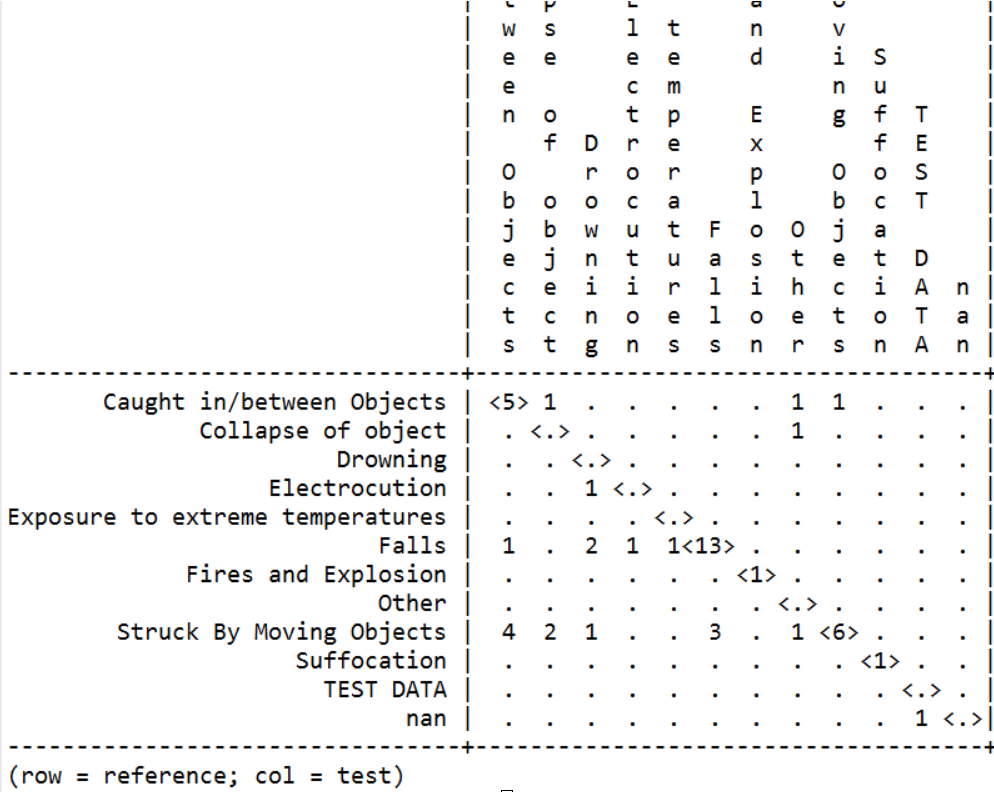
\includegraphics[width=0.3\textwidth]{confusion.png}
  \caption{Confusion Matrix}
\end{figure}

Below is the classification report of the test data. We can see the
precision, recall, fi-score and support value of the built model.


\begin{figure}[h!]
  \centering
      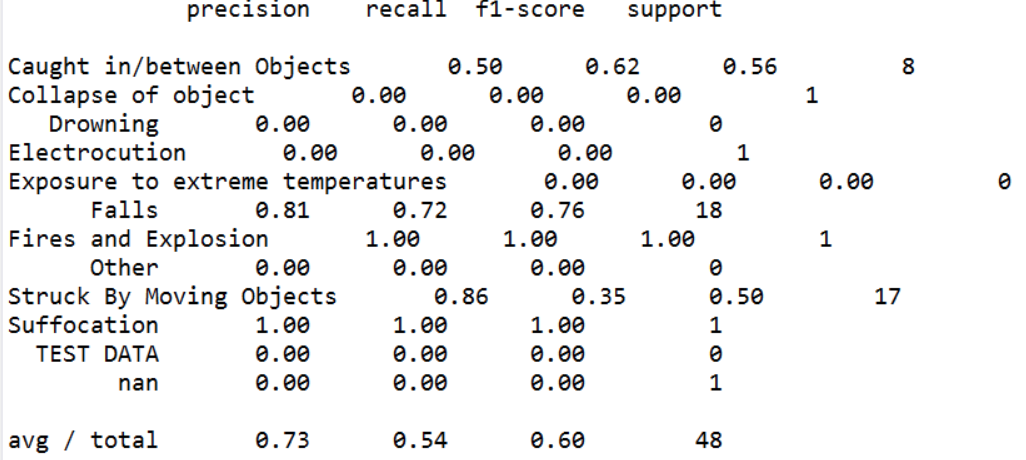
\includegraphics[width=0.5\textwidth]{class_report.png}
   \caption{Classification Report}
\end{figure}

\subsection{Prediction}

Do classification about the accident cause of the osha.csv data. There
are several columns of the osha.csv data. We use only the summary
column. Transform the new data features to fit the already trained
TF-IDF. Then use the trained model on the new data. A part of the
classification results are shown as follows.

\begin{figure}[h!]
  \centering
      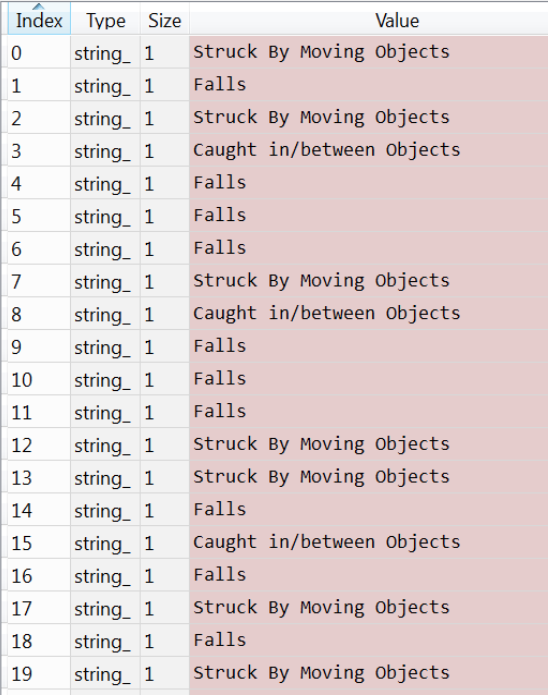
\includegraphics[width=0.2\textwidth]{class_result.png}
   \caption{Classification Result}
\end{figure}

\section{Objects of Accident}
In this task, we used some different tools in nltk to help us find out
the statistics of different objects causing an accident.


The approach we use to tackle this problem is to train a regular
expression chunker which extracts the objects that cause the
accidents.

\subsection{Data Preprocessing}
After examine the text data in “Title Case” column, we found that,
there is certain syntactic structure of the text, i.e. the target
objects which cause the accident appear after a proposition or
“to”. E.g. “Employee Injures Self With Knife”, the object causes the
accident is “knife”, and it appears after a proposition
“with”. Therefore, we can use this pattern to extract the target
objects.

Also there are a lot of error messages ' InspectionOpen
DateSICEstablishment Name', we eliminated these messages with some
simple script.

We found that the first character of each word in the sentence is
capitalized and it causes problems when we try to POS tag the text. So
normalizing each word to small letter is required.


\subsection{POS Tagging}
After data exploration and preprocessing, we POS tag each record of
“Title Case” to get the POS tags so that we can use regular expression
to extract the target objects later.

After data exploration and preprocessing, we POS tag each record of
“Title Case” to get the POS tags so that we can use regular expression
to extract the target objects later. Below is an example of POS tagged
record, as can be seen, the target object “forklift” (NN) is after
“by” (IN).


\subsection{Regular Expression}
After POS tagging, we build a regular expression based chunk parser,
for each record of “Title Case”, we extract the target object.

We calculate the frequency of each object and list the top objects
(as shown below) with the highest frequency.

From the result, we can see that the most frequent object is ‘fall’
which actually is not an ‘object’, so we sort the top 11 from the
result, and got the top 10 objects and their frequency respectively.


\begin{figure}[h!]
  \centering
      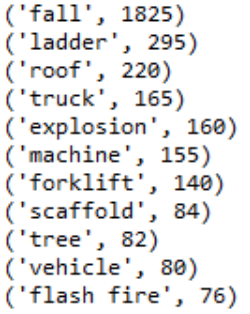
\includegraphics[width=0.2\textwidth]{obj11.png}
   \caption{Top Objects}
\end{figure}

The final top 10 objects and there frequencies are {\bf ladder, roof,
  truck, explosion, machine, forklift, scaffold, tree, vehicle, flash fire.
}

In order to provide a more intuitive way to view our result we made a
wordnet, shown as Figure. 5.


\begin{figure}[h!]
  \centering
      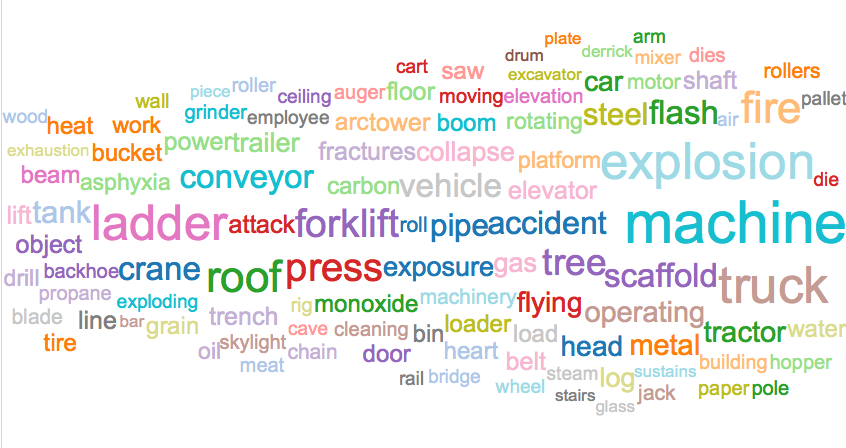
\includegraphics[width=0.4\textwidth]{common_objects.png}
   \caption{Common Objects That Causes Accidents}
\end{figure}


Due to the complexity of the syntactic structure, one simple regular
expression can’t identify all target objects in records, as we can see
from the result, the top one object found by the chunk parser is
‘fall’ which appears 1825 times, however, ‘fall’ may or may not be
considered as an object which causes the accident, so manual
examination of the result is quite necessary. To further improve the
accuracy, we can analyze the syntactic structure of each record more
carefully and come up with more sophisticated regular expression or
try more complex parser, e.g. dependency parser, etc.



\section{Occupations}

Finding occupations that are more risky contains work of finding
highly frequently appearing subject of all accident descriptions.

\subsection{Data Preprocessing}
We made some modifications in the two tables. For this task we mainly
used osha.csv. Some of the types are not consistent with the titles
and summary contents. We correct them according to the title and
summary content. Besides there are other and others in the type
list. We change them to other to make it uniform.


\subsection{POS Tagging and Results}

For this task the POS tagging is almost the same with the one in
Chapter. 2. Here we reduce the process of explaining: when extracting
subject of an accident, the subject(noun) will be considered as the
occupation.

After we run the test we got the following occupations as the most
frequently involved in accidents:

{\bf $$\small Employee, Worker, Operator, Carpenter,$$
$$Driver, Mechanic, Installer,$$
$$Foreman, Zookeeper$$}

There might be inaccuracy with the result, further research will cover
how to increase the accuracy.


\section{Common Activities}

For finding the common activities we are using the “summary” column in
osha dataset. Which provides detailed information about the incident
which caused the accident, including what happened prior to the
accident.


\subsection{Data Preprocessing}

As we know the activities are mentioned in the first sentence of every summary case, we are going to limit the number of lines to the first, also it will help us to reduce the complexity involved in computation and POS tagging. Furthermore, we can avoid dealing with secondary or detailed information is given later sentences.
We also removed the empty rows as they won’t be contributing towards
the results.




\subsection{POS Tagging and Chunking}

To get the part of sentence which involves the user activity we are
going to perform chunking, Grammar for chunking the activity, and
represented in past continuous tense, and ends with noun phrase.

n our chunk there are many english stopwords which are causing the activities to be non consistent, we will be removing all english stopwords.


For indicating the activity we will only look into the sentences which have words with *.ing. This
gives us the chunks which contain actions along with the things which they were envolved with

\subsection{Finding Activities}
In the end we will be only extracting the actions the persons were involved in by using
POS tagging and grammar as
$$grammar = r"""{<VBG|JJ>+}"""$$
This gives us all the actions the they performed.


\begin{figure}%
    \centering
    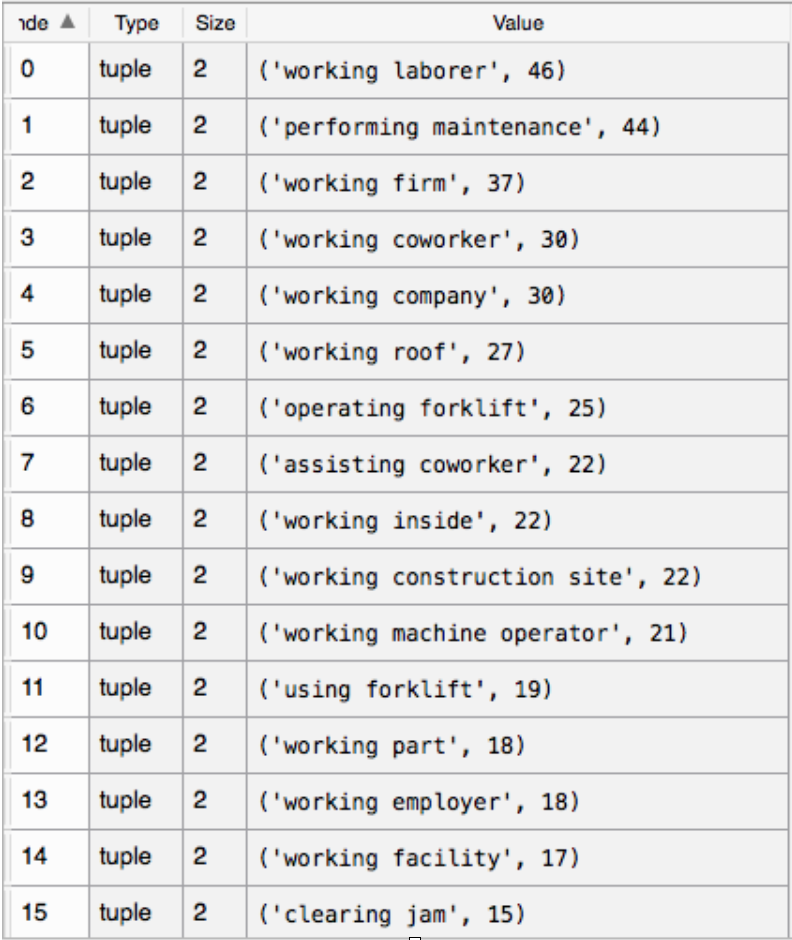
\includegraphics[width=4cm]{q41.png}
    %\qquad
    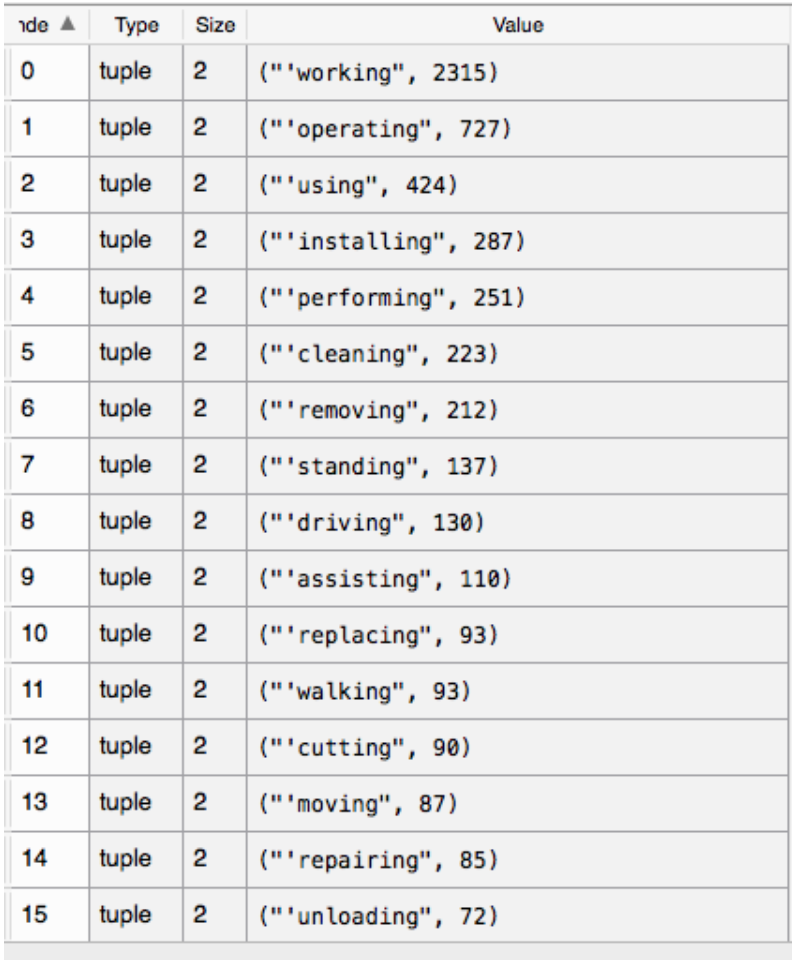
\includegraphics[width=4cm]{q42.png}
    \caption{(Left)Common Action Involved Together with Relavent
      People. (Right)Common Actions before Accidents.}%
\end{figure}


The following word nets are to show the word frequency:

\begin{figure}[h!]
  \centering
      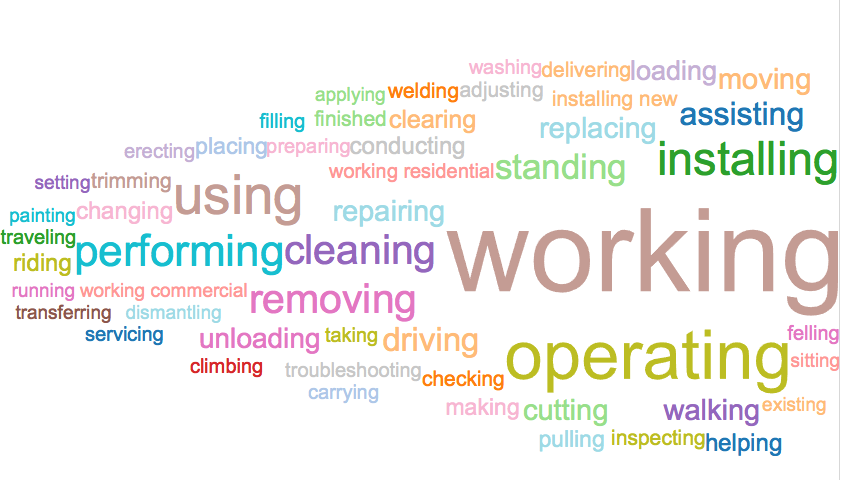
\includegraphics[width=0.5\textwidth]{bef_acc.png}
   \caption{Common Activities before Accident}
\end{figure}


\begin{figure}[h!]
  \centering
      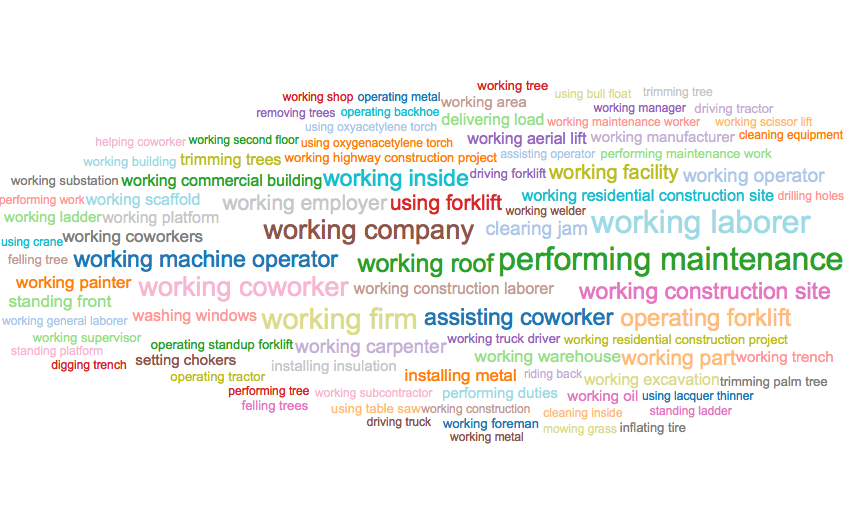
\includegraphics[width=0.5\textwidth]{act.png}
   \caption{Common Activities}
\end{figure}


\section{Conclusion}

Use SVM algorithm to build classification model to find out type of
accidents (in terms of main causes) which are more common in fatal or
catastrophic accidents of the osha data.

The common activities in which person was involved could be found.
Also we can get the things involved and other culprit for the
accidents by the chunking.

However, even though we found common actions, but they are not summarized very well.
the number of actions in which we can clearly pinpoint what person was
doing, but we fail to get comparable numbers when we are trying to
pinpoint the.

While capturing only if we asked the operator to put a generic action,
which could be a list of 30-50 activities which are predefined and
then we can also further ask the subcategory. This will resolve the
issue of inconsistent text values.

We can import the results provided here into visualization or other analytical tool to further analyse the issues.
Current results can also be used as things during which worker should
be careful with and we can also recommend the precautions to be taken.

Try with more than one sentence from summary case to see the results.
Also try using the n-gram approach while performing the chunking.


\bibliographystyle{plain}
\bibliography{sample}{}

%----------------------------------------------------------------------------------------

\end{document}
%%% Local Variables:
%%% mode: latex
%%% TeX-master: t
%%% End:
